\chapter{\IfLanguageName{dutch}{Stand van zaken}{State of the art}}%
\label{ch:stand-van-zaken}

% Tip: Begin elk hoofdstuk met een paragraaf inleiding die beschrijft hoe
% dit hoofdstuk past binnen het geheel van de bachelorproef. Geef in het
% bijzonder aan wat de link is met het vorige en volgende hoofdstuk.

% Pas na deze inleidende paragraaf komt de eerste sectiehoofding.

\section{Inleiding}
\label{sec:stand-van-zaken-inleiding}

In dit deel van de bachelorproef worden de zonnepanelen, de laadpaal, het beluchtingssysteem van het water, de protocollen, de data registers, de backend en de front-end besproken. De reden hiervoor is dat er grondig onderzocht wordt hoe alle componenten kunnen samenwerken en een diepere kennis te krijgen van deze componenten. In afbeelding \ref{fig:Netwedrkdiagram-Opstelling} wordt een visualisatie van de opstelling weergegeven, met de belangrijkste verbruikers en producenten.

\begin{figure}[h]
    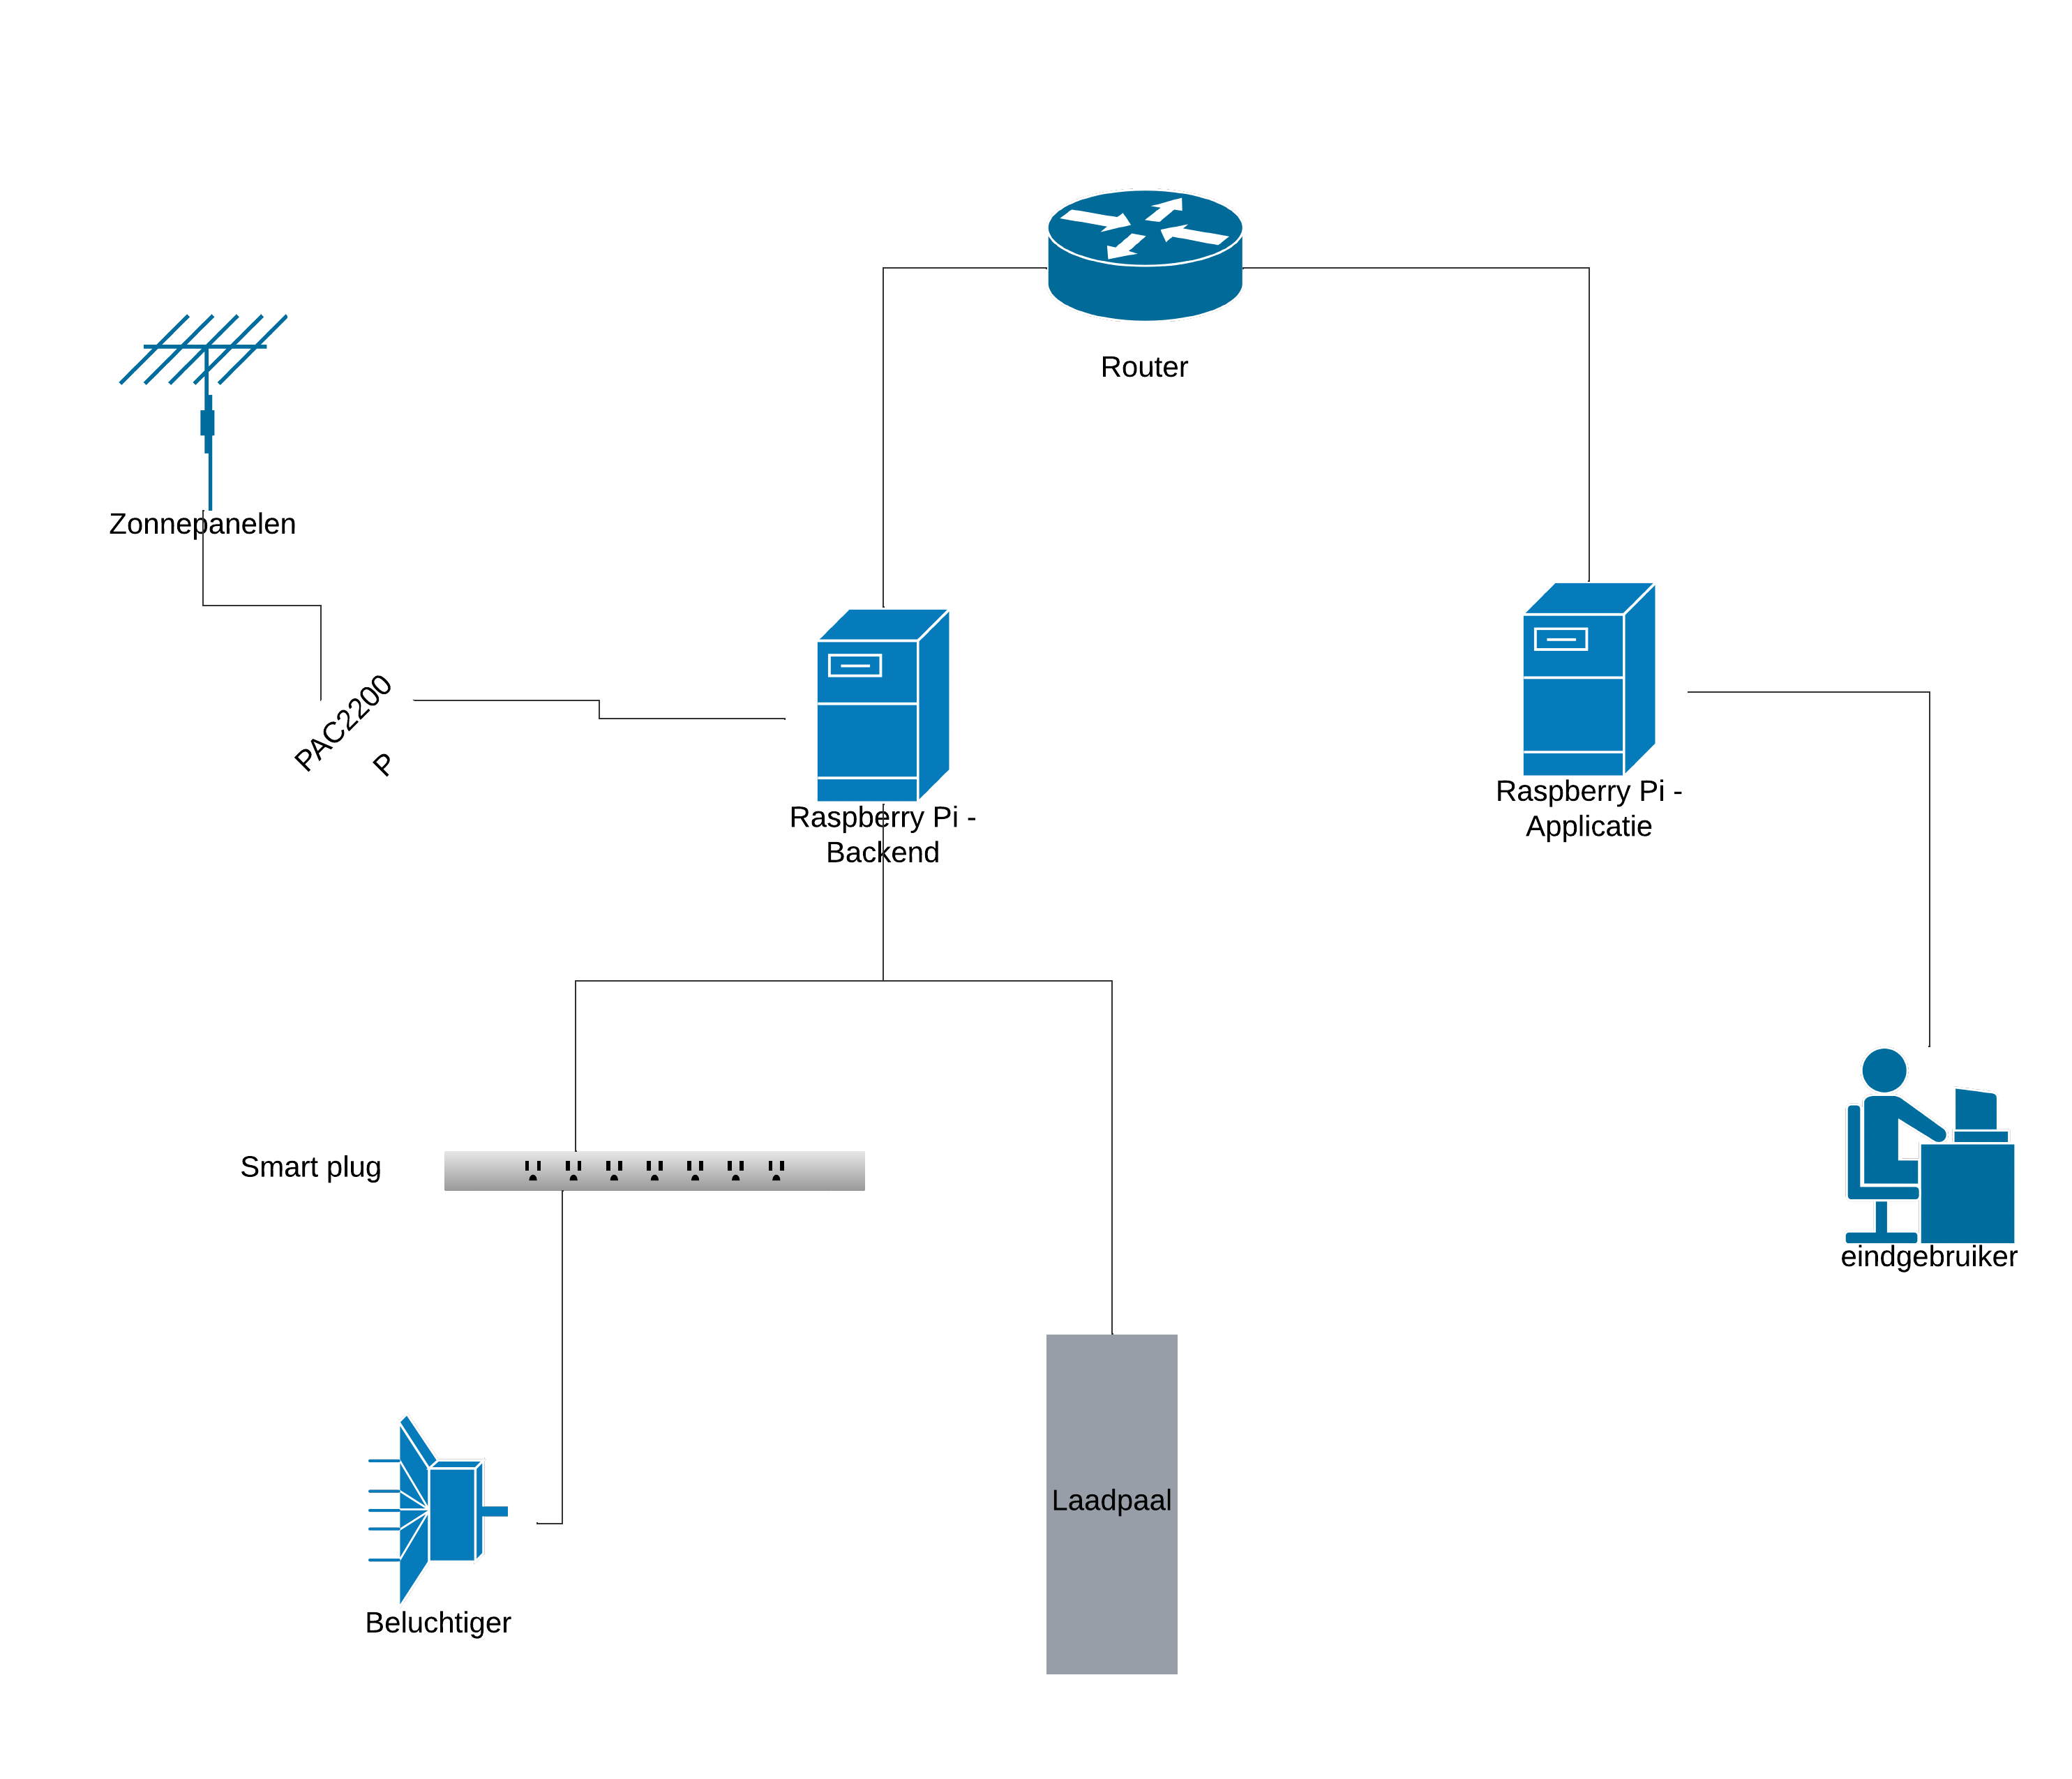
\includegraphics[width=10cm]{./graphics/Netwerkdiagram-Opstelling.png}
    \caption{grafische voorstelling van de proefopstelling.}
    \label{fig:Netwedrkdiagram-Opstelling}
\end{figure}

\section{Zonnepanelen}
\label{sec:stand-van-zaken-zonnepanelen}

Carwash Clean Car heeft sinds 2013 zonnepanelen. Deze zonnepanelen zijn geplaatst om de maandelijkse elektriciteitsfactuur te verlagen. Maar de laatste jaren merkt het bedrijf op dat de maandelijkse elektriciteitsfactuur terug begint te stijgen, de oorzaak van deze stijging is dat er op momenten te weinig elektriciteit wordt opgewekt met de zonnepanelen om alle elektriciteit intensieve bedrijfsprocessen aan te sturen. Nu is het de bedoeling om de data van de zonnepanelen uit te lezen, om zo de niet-dringende elektriciteit intensieve bedrijfsprocessen aan te sturen wanneer er genoeg elektriciteit wordt opgewekt met deze zonnepanelen.\\ Het bedrijf Carwash Clean Car heeft in totaal 432 ET-Solar zonnepanelen op hun domein. Het piekvermogen van 1 zonnepaneel bedraagt 235 Watt piek, dus alle panelen samen zorgen dan voor een piekvermogen van 101 520 Watt piek. Om de opgewekte zonne-energie om te zetten naar elektriciteit zijn er ook omvormers nodig, hiervoor maakt de carwash gebruik van deze omvormers:

\begin{itemize}
    \item ABB Trio 27,6 TL (2x geïnstalleerd)
    \item SMA Tripower 15000 TL (1x geïnstalleerd)
    \item SMA Tripower 17000 TL (1x geïnstalleerd)
\end{itemize}

In het jaar 2023 worden in totaal 61 417 kilowattuur aan zonne-energie geproduceerd in Carwash Clean Car. Van deze 61 417 kilowattuur , was 34 316 kilowattuur overtollig, deze energie werd dan terug op het net geïnjecteerd. Er zijn ook momenten dat er te weinig energie wordt opgeleverd via de zonnepanelen, hierdoor is er ook aan 33 223 kilowattuur elektriciteit aangekocht. In afbeelding \ref{fig:energie-productie-2023} kan worden waargenomen dat er de wintermaanden veel meer elektriciteit geïmporteerd moet worden, in de zomer zal er dan weer meer energie geëxporteerd moeten worden. De geïmporteerde energie is vanaf het nulpunt tot + oneindig, de opgewekte energie is vanaf het nulpunt tot - oneindig.

\begin{figure}[h]
    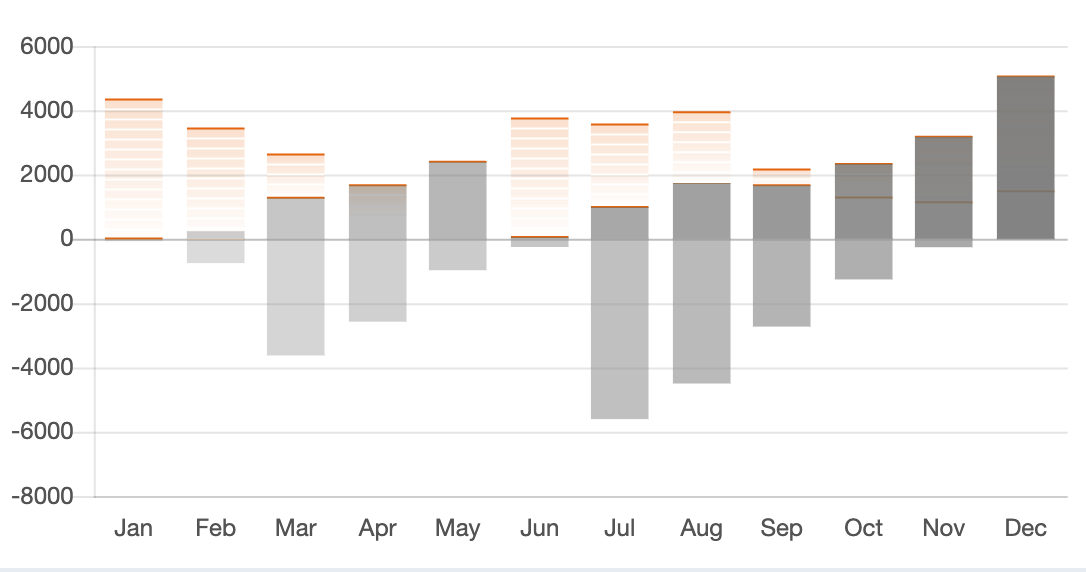
\includegraphics[width=10cm]{./graphics/Energie-opbrengsten-2023}
    \caption{Een grafiek van de aankoop en productie van elektriciteit in 2023.}
    \label{fig:energie-productie-2023}
\end{figure}

Voor het uitlezen van de hoeveelheid energie die wordt opgewekt met de zonnepanelen zijn er verschillende componenten nodig. Een van de belangrijkste componenten is de omvormer. Dit component zorgt ervoor dat de opgewekte energie van de zonnepanelen omgezet kan worden in elektriciteit. Nadat de energie is omgezet naar elektriciteit gaat er via de Siemens PAC2200 monitoring gebeuren, deze monitoring is een realtime uitlezing van de opgewekte en aangekochte elektriciteit. De reden dat de Siemens PAC2200 gebruikt wordt in de proefopstelling, is omdat deze al geïnstalleerd staat in de carwash. Aangezien de uitlezing gebeurt door de Siemens PAC2200 aan te spreken, moet er gekeken worden welke protocollen dit apparaat ondersteunt. De communicatieprotocollen  kunnen teruggevonden worden bij de subtitel Ethernet onderaan pagina 28 van de handleiding van dit product van siemens \footnote{Deze informatie is teruggevonden op deze website: \url{https://cache.industry.siemens.com/dl/files/681/109476681/att_108732/v1/SITRANS_PAC2200_UM_EN-US_A6V1020.pdf}. De handleiding is geraadpleegd op 17 april 2024}:

\begin{itemize}
    \item Modbus TCP
    \item Web Server (HTTP)
    \item SNTP
    \item DHCP
\end{itemize}

Het enige protocol dat ook door de omvormers ondersteund wordt is Modbus TCP, dus dit is het protocol dat gebruikt gaat worden in de proefopstelling. In sectie \ref{sec:stand-van-zaken-protocollen} wordt er meer toegelicht over de functies van het Modbus TCP protocol.\\ 

Als er een connectie gemaakt is met Siemens PAC2200, wordt de waarde van de opgewekte en aangekochte elektriciteit doorgestuurd naar de backend. Zo kan er berekend worden of er genoeg elektriciteit beschikbaar is om bepaalde energie-intensieve bedrijfsprocessen te starten.\\

Aan de hand van de opgehaalde data zullen er verschillende diagrammen beschikbaar gesteld worden, zodat de eindgebruiker kan kiezen hoe deze data weergeven wordt. Om de data makkelijk op te halen in de applicatie zal deze verbonden worden met de backend. De backend wordt in sectie \ref{sec:stand-van-zaken-backend} verder toegelicht.

\section{laadpaal}
\label{sec:stand-van-zaken-laadpaal}

Één van de niet-dringende bedrijfsprocessen dat aangestuurd moet worden is het laden van de elektrische voertuigen met de laadpaal. Er bestaan verschillende laadpalen voor elektrische voertuigen. Momenteel wordt er één laadpaal gebruikt bij het bedrijf. Deze laadpaal is namelijk de Eve Single S-line van Alfen. Deze laadpaal maakt gebruik van een type 2 connector. "Dit type is de IEC 62196-2 standaard dat gebruikt wordt in Europa. Deze standaard kan tot 43 kilowatt snel laden en wordt voornamelijk gebruikt voor openbare laadpalen. Er bestaat ook een type 1 connector, dit is de standaard connector in Amerika en Azië." \autocite{HEMAVATHI2022105013} \\

De laadpaal van het bedrijf kan tot 11 kilowatt snel laden. Volgens de datasheet van Alfen \footnote{Deze informatie is teruggevonden op deze website: \url{https://alfen.com/nl-be/file-download/download/public/2753}. De handleiding is geraadpleegd op 17 april 2024} heeft de geïnstalleerde laadpaal ook de mogelijkheid om slim te laden, hiervoor zijn er verschillende ingangen beschikbaar, deze zijn:

\begin{itemize}
    \item DSMR 4.0-4.2 en SMR5.0
    \item Externe relais
    \item Modbus TCP/IP (externe kilowattuur meter)
    \item Modbus TCP/IP Slave (energiebeheersysteem)
    \item Modbus RTU (externe kilowattuur meter)
    \item Télé-information client (slimme meter linky)
\end{itemize}

Aangezien er een webapplicatie gemaakt zal worden en deze applicatie een energiebeheersysteem zal worden, wordt er een Modbus TCP/IP Slave connectie gebruikt. Op de website van Alfen is een document beschikbaar gesteld waar een lijst in staat met alle data registers die gebruikt kunnen worden.\\

Voor het uitlezen van de laadpaal is er niet veel nodig, omdat deze al op het internet is aangesloten en er een Modbus TCP/IP Slave connectie op geïnstalleerd staat. Het enige wat er moet gebeuren is het IP-adres opzoeken van de laadpaal in de router en de juiste data registers opzoeken in de handleiding die op de website van Alfen beschikbaar gesteld staat. Als deze gegevens geweten zijn, kan er via de backend een connectie gelegd worden met de laadpaal.\\

Zoals eerder vermeld zijn er verschillende connectie types beschikbaar op de laadpaal. Het type dat gebruikt gaat worden is een Modbus TCP/IP Slave connectie. Later in sectie \ref{sec:stand-van-zaken-protocollen} wordt er meer toegelicht over de werking van het Modbus TCP/IP Slave protocol.\\

Om de juiste data uit de laadpaal te halen en de laadpaal juist aan te sturen zal er ook geweten moeten zijn welke registers er aangesproken moeten worden. De meeste registers van deze laadpaal worden weergegeven in numerieke waarden, maar er zijn ook een paar registers aan te spreken waar de waarde als een string weergegeven wordt. Het precieze data type staat in de kolom Data Type van de tabel in de handleiding van Alfen\footnote{Deze informatie is teruggevonden op deze website: \url{https://alfen.com/file-download/download/public/1610}. De handleiding is geraadpleegd op 17 april 2024}.\\

De data zal makkelijk op te halen zijn via de backend die geconnecteerd is met de laadpaal. Deze backend stuurt dan de juiste data door naar de webapplicatie. De webapplicatie zal via de backend kijken of de laadpaal actief is, als deze actief is zal er een schakelaar zijn die dit aantoont. Er zal ook een optie zijn om via een dropdown menu te selecteren op welk vermogen de laadpaal moet laden. De laadpaal zal ook automatisch ingeschakeld worden als er genoeg overschot is aan groene energie, zo moet de eindgebruiker de webapplicatie niet altijd in de gaten houden om de laadpaal in te schakelen.

\section{Beluchtingssysteem van het water}
\label{sec:stand-van-zaken-beluchtingssysteem}

Het bedrijf Carwash Clean Car zuivert een deel van het water dat er gebruikt wordt in de carwash zelf, hierdoor is er ook een beluchtingssysteem geïnstalleerd. Dit beluchtingssysteem verbruikt niet zo veel elektriciteit en moet niet continu aan staan, daarmee kwam de vraag of deze ook smart aangestuurd kon worden aan de hand van een smart plug.\\

Het beluchtingssysteem van het water verbruikt 3 kilowatt als deze aan het werken is. Dit is niet veel, maar het is niet dat dit fluctueert tussen 0 kilowatt en 3 kilowatt. Het verbruikt dus continu 3 kilowatt.\\

Voor het beluchtingssysteem slim aan te sturen is er een smart plug voorzien, deze smart plug zal verbonden zijn met het internet om aangestuurd te kunnen worden. Via de webapplicatie zal er een booleaanse waarde doorgestuurd worden naar de backend. De backend zal dan op zijn beurt, aan de hand van de booleaanse waarde, een signaal doorsturen naar de smart plug om deze aan of af te zetten.\\

Om het aansturen van het beluchtingssysteem gebruiksvriendelijk weer te geven, wordt aan de hand van een schakelaar in de applicatie weergegeven of de smart plug aan of uit staat. Zo kan de gebruiker zelf kiezen wanneer deze aan of uit moet staan.

\section{protocollen}
\label{sec:stand-van-zaken-protocollen}

Aangezien er verschillende protocollen nodig zijn voor de apparaten, zoals de zonnepanelen en de laadpaal aan te spreken, worden deze hier uitgebreider besproken. De reden hiervoor is dat er een grondige voorkennis wordt opgedaan over de protocollen die gebruikt kunnen worden.\\

De protocollen die gebruikt gaan worden zijn versies van het Modbus protocol. Zo wordt voor de zonnepanelen Modbus TCP/IP gebruikt en voor laadpaal zal Modbus TCP/IP Slave connectie gebruikt worden.\\

"Het Modbus protocol is ontwikkeld in 1979 door Modicon, het werd oorspronkelijk ontwikkeld om industriële automatisering en Modicon controllers te programmeren. Sindsdien is het Modbus protocol een industrie standaard geworden voor het overdragen van discrete analoge I/O informatie en het registreren van data tussen industriële controle en monitoring apparaten." \autocite{Acromag2005} \\

"Apparaten die het Modbus protocol gebruiken om te communiceren, maken gebruik van een master-slave (client-server) techniek, waarin enkel 1 apparaat (de master of client) de transacties (anders verwoord queries) kan beginnen. De andere apparaten (slaves of servers) antwoorden door de gevraagde data door te geven aan de master, of door de actie door te voeren dat gevraagd werd in de query." \autocite{Acromag2005} \\

"Het Modbus TCP/IP ook wel Modbus-TCP genoemd protocol is het Modbus protocol met een TCP interface dat op ethernet draait." \autocite{Acromag2005} In afbeelding \ref{fig:modbus-data-pakket} wordt de constructie van een Modbus TCP Data pakket weergegeven.\\

Voor de laadpaal wordt het Modbus TCP/IP Slave protocol toegepast, wat wil zeggen dat de backend de master is en de laadpaal de slave die de data voorziet aan de backend.

\begin{figure}[h]
    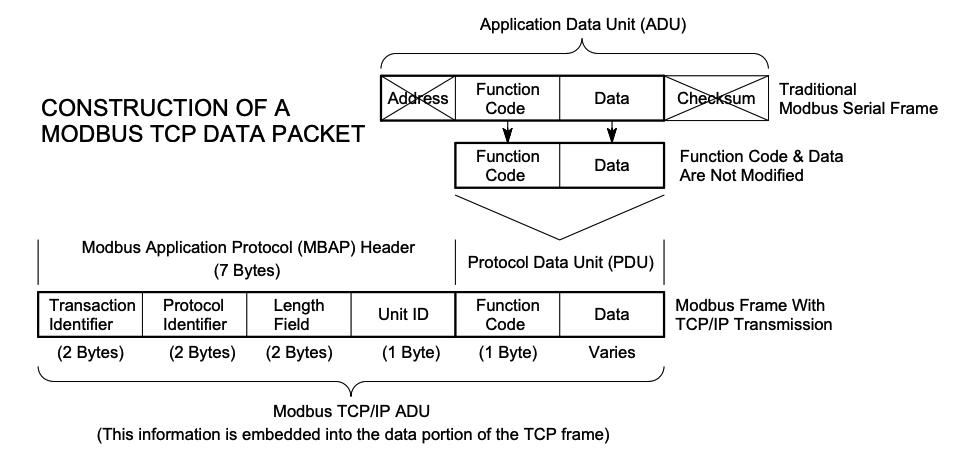
\includegraphics[width=10cm]{./graphics/Modbus-TCP-schema.png}
    \caption{Een grafische voorstelling van een Modbus TCP Data pakket. \autocite{Acromag2005}}
    \label{fig:modbus-data-pakket}
\end{figure}

\section{dataregisters}
\label{sec:stand-van-zaken-dataregisters}

\section{Backend}
\label{sec:stand-van-zaken-backend}

\section{Webapplicatie}
\label{sec:stand-van-zaken-webapplicatie}
